\chapter{評価}
\label{chap:eval}
ランサムウェアによる暗号化からデータを保護する性能と,Fuga稼働時のオーバーヘッドを評価した.
評価はすべて\tabref{tab:experiment-machine-kashiwa}に示す物理マシン上で行った.
\begin{table}[t]
  \caption{Environment of the physical machine used for the evaluation.}
  \label{tab:experiment-machine-kashiwa}
  \hbox to\hsize{\hfil
    \begin{tabular}{l|lll}
      \hline \hline
      OS       & Ubuntu 22.04.4 LTS                                  \\
      ファイルシステム & ext4                                                \\
      カーネル     & 6.3.0-060300-generic                                \\
      CPU      & \scriptsize{Intel Xeon Silver 4314 @ 2.400GHZ × 64} \\
      RAM      & 512GiB                                              \\ \hline
    \end{tabular}\hfil}
\end{table}

\section{データ保護性能の評価}
\subsection{実験シナリオ}
指定されたパスのファイルを\texttt{read}し,OpenSSL内の関数で暗号化したのち新規ファイルに\texttt{write}するプログラムをC言語で実装した.
暗号化方式はAES256を使用し,鍵長とIV長はそれぞれ32Bと16Bとした.\texttt{read}などの処理は4096Bのバッファに対して行うようにした.
このプログラムをこれ以降「\textbf{暗号化プログラム}」と称する.

OpenSSLが提供するコマンドを使用して,指定したバイト長の擬似乱数を含むファイルを生成する.
そして生成したファイルに対して以下の手続きを行う.
\begin{enumerate}
  \item 実装した提案手法を実行する.
  \item 暗号化プログラムでファイルを暗号化する.
  \item 元のファイルと,Data Shelter内に作成されたファイルを用いて評価を行う.
\end{enumerate}
暗号化の対象となるファイルを「\textbf{元ファイル}」,Data Shelter内に作成されるファイルを「\textbf{退避ファイル}」と呼ぶ.

この実験におけるデータ保護性能の評価指標として,\textbf{一致率}を定義した.
一致率は,退避ファイルと元ファイルがどの程度一致しているかを表す指標である.
元ファイルと退避ファイルのデータをバイト値の配列とみなし,先頭から配列の値を調べて一致している個数を数え,
その個数を元ファイルのバイトサイズで割ると一致率が求められる.
元ファイルが\texttt{[1, 2, 3, 4, 5]},退避ファイルが\texttt{[1, 2, 4]}の場合,先頭の1と2が一致しているので
この時の一致率は$\frac{2}{5}=0.4$である.

\subsection{予備実験の結果}
\label{subsec:preliminary-result}
先行研究\cite{css2024}で示した実装をによる提案手法の一致率を予備実験で評価した.
結果を\figref{fig:seq-vs-par-exp}および\figref{fig:seq-vs-par-inc}に示す.
Evacuation Moduleが実行する3つの処理Read,Decode,Writeのそれぞれの処理時間の分布を\figref{fig:elapsed-time}に示す.
\begin{figure}[h]
  \centering
  \begin{minipage}[b]{0.49\columnwidth}
    \centering
    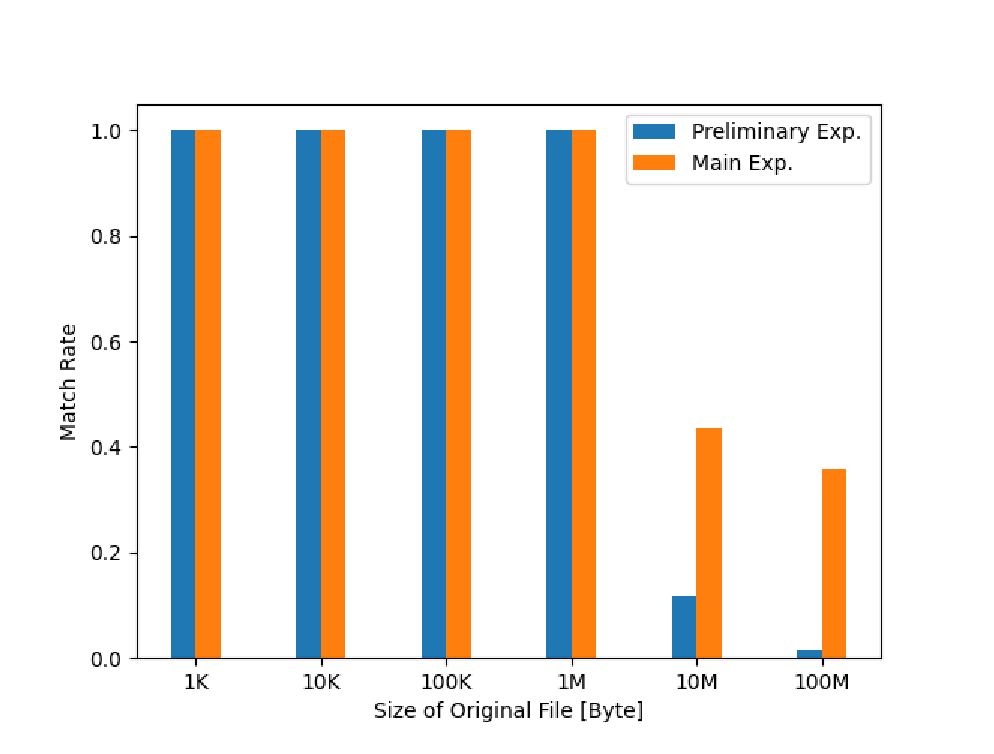
\includegraphics[width=\columnwidth]{doc/img/eval/seqential_vs_parallel_match_p4_exp.eps}
    % \caption{Match rates by original file size. The horizontal axis is presented on a common logarithmic scale,
    % comparing results from the preliminary and main experiments.}
    \caption{tmp}
    \label{fig:seq-vs-par-exp}
  \end{minipage}
  \begin{minipage}[b]{0.49\columnwidth}
    \centering
    \includegraphics[width=\columnwidth]{doc/img/eval/seqential_vs_parallel_match_p4_inc.eps}
    % \caption{Match rates by original file size,
    % comparing results from the preliminary and main experiments.}
    \caption{foobar}
    \label{fig:seq-vs-par-inc}
  \end{minipage}
  \caption{Match rates by original file size, comparing results from the preliminary and main experiments.
    The horizontal axis in the left figure uses a common logarithmic scale.}
\end{figure}

\begin{figure}[t]
  \begin{center}
    \includegraphics[width=\columnwidth]{doc/img/eval/hakohige_sequential.eps}
  \end{center}
  \caption{Boxplot of processing times for the three operations in the Evacuation Module: Read, Decode, and Write.
    Entries with processing times exceeding 1000 µs were excluded; only 2 out of 976 total entries were removed.}
  \label{fig:elapsed-time}
\end{figure}

\subsection{元ファイルのサイズに対する一致率の変化}
本稿では先行研究 \cite{css2024} と同様に,
1KB,10KB,$\ldots$,100MBのサイズの元ファイルに対して実験を行い,一致率を計算した.
Decode処理の並列度は4に,リングバッファのサイズは1MiBに設定した.
その結果を\figref{fig:seq-vs-par-exp}に示す.
また,1MBから10MBまで1MB刻みのサイズのファイルを生成し実験を行った.並列度とリングバッファの設定は同一である.
結果を\figref{fig:seq-vs-par-inc}に示す.
先行研究 \cite{css2024} で示された一致率からの向上が確認され,
高速化,すなわちEvacuation Moduleのパイプライン化とデコード処理の並列化,が保護性能の改善に寄与したことがわかった.
性能改善の程度は元ファイルのサイズが大きいほど顕著であり,100MBの元ファイルに対しては20倍以上の差が見られた.
